In this section we evaluate the performance of our work-stealing framework built upon SALSA pools. 
We describe the experiment setup in Section~\ref{sec:exp-setup}, we show the overall system performance in Section~\ref{sec:eval-performance} and study the influence of various SALSA techniques in Section~\ref{sec:eval-techniques}.

\subsection {Experiment Setup}
\label{sec:exp-setup}
The implementation of the work-stealing framework used in our evaluation does not include the linearizability mechanisms described in~\ref{alg-safety}. We believe that these mechanisms have negligible effect on performance, moreover, in our simulations they are never invoked because the pool is never empty. We compare the following task pool implementations:
\begin {itemize}
\item
{\bf WS-SALSA} -- our work-stealing framework with SCPools implemented by SALSA.
\item
{\bf WS-SALSAwCAS} -- our work-stealing framework with SCPools implemented by a simplistic SALSA variation, in which every {\bf consume()} and {\bf steal()} operation tries to take a single task using CAS. In essence, SALSAwCAS removes the effects of SALSA's low-synchronization fast-path and per-chunk stealing. 
Note that disabling per-chunk stealing in SALSA annuls the idea of chunk ownership, hence, removing the per-chunk stealing mechanism in SALSA implies disabling its low-synchronization fast-path as well. 
\item
{\bf ConcBag} -- an algorithm similar to the lock-free Concurrent Bags algorithm~\cite{Sundell:2011:LAC:1989493.1989550}. 
No thread in our system acts as both a producer and a consumer, therefore every consume operation of a Concurrent Bags algorithm steals a task from some producer.
We did not have access to the original code, and therefore reimplemented the algorithm in our framework. Our implementation is faithful to the algorithm in the paper, except in using a simpler and faster linked list algorithm. All engineering decisions were made to favor the original algorithm. 
\item
{\bf WS-MSQ} -- our work-stealing framework with SCPools implemented by Michael-Scott non-blocking queue~\cite{Michael:1996:SFP:248052.248106}. Both {\bf consume()} and {\bf steal()} operations invoke the {\bf dequeue()} function of the queue. 
\item
{\bf WS-LIFO} -- our work-stealing framework with SCPool implemented by LIFO stack by Michael~\cite{Michael:2004:HPS:987524.987595}. 
\end {itemize} 

We did not implement our work-stealing framework with other FIFO and LIFO queue implementations, because, as it was shown in~\cite{Sundell:2011:LAC:1989493.1989550}, their performance is the same order of magnitude with Michael-Scott queue. 
We also did not evaluate {CAF\'E} pools because their performance is similar to that of WS-MSQ~\cite{Basin:Thesis:2011}, and ED-Pools~\cite{Afek:2010:SPP:1885276.1885295}, which have been shown to scale poorly in the multi-processor architectures~\cite{Basin:Thesis:2011,Sundell:2011:LAC:1989493.1989550}. 

All the pools are implemented in C++ and compiled with \texttt{-O2} optimization level. 
In order to minimize the scalability issues related to the excessive memory allocations, we use \texttt{jemalloc} allocator~\cite{citeulike:4951109}, which has been shown to be highly scalable in multi-threaded environments\footnote{\url{http://www.facebook.com/notes/facebook-engineering/scalable-memory-allocation-using-jemalloc/480222803919}}.
Unless stated otherwise, chunks of SALSA and SALSAwCAS contain $1000$ tasks, and chunks of ConcBag contain $128$ tasks, which were the optimal values for each algorithms. 

We use a synthetic benchmark for performance evaluation, where 1) each producer works in a loop of inserting dummy items; 2) each consumer works in a loop of retrieving dummy items. Each data point shown is an average of $5$ runs, each with a duration of $20$ seconds. 
The tests are run on a dedicated shared memory NUMA server with $8$ Quad Core AMD $2.3$GHz processors and $16$GB of memory attached to each processor. 

\subsection{System Throughput}
\label{sec:eval-performance}

\begin{figure}[htb]
	\centering
  \subfigure [\scriptsize{System throughput -- N producers, N consumers.}] {
    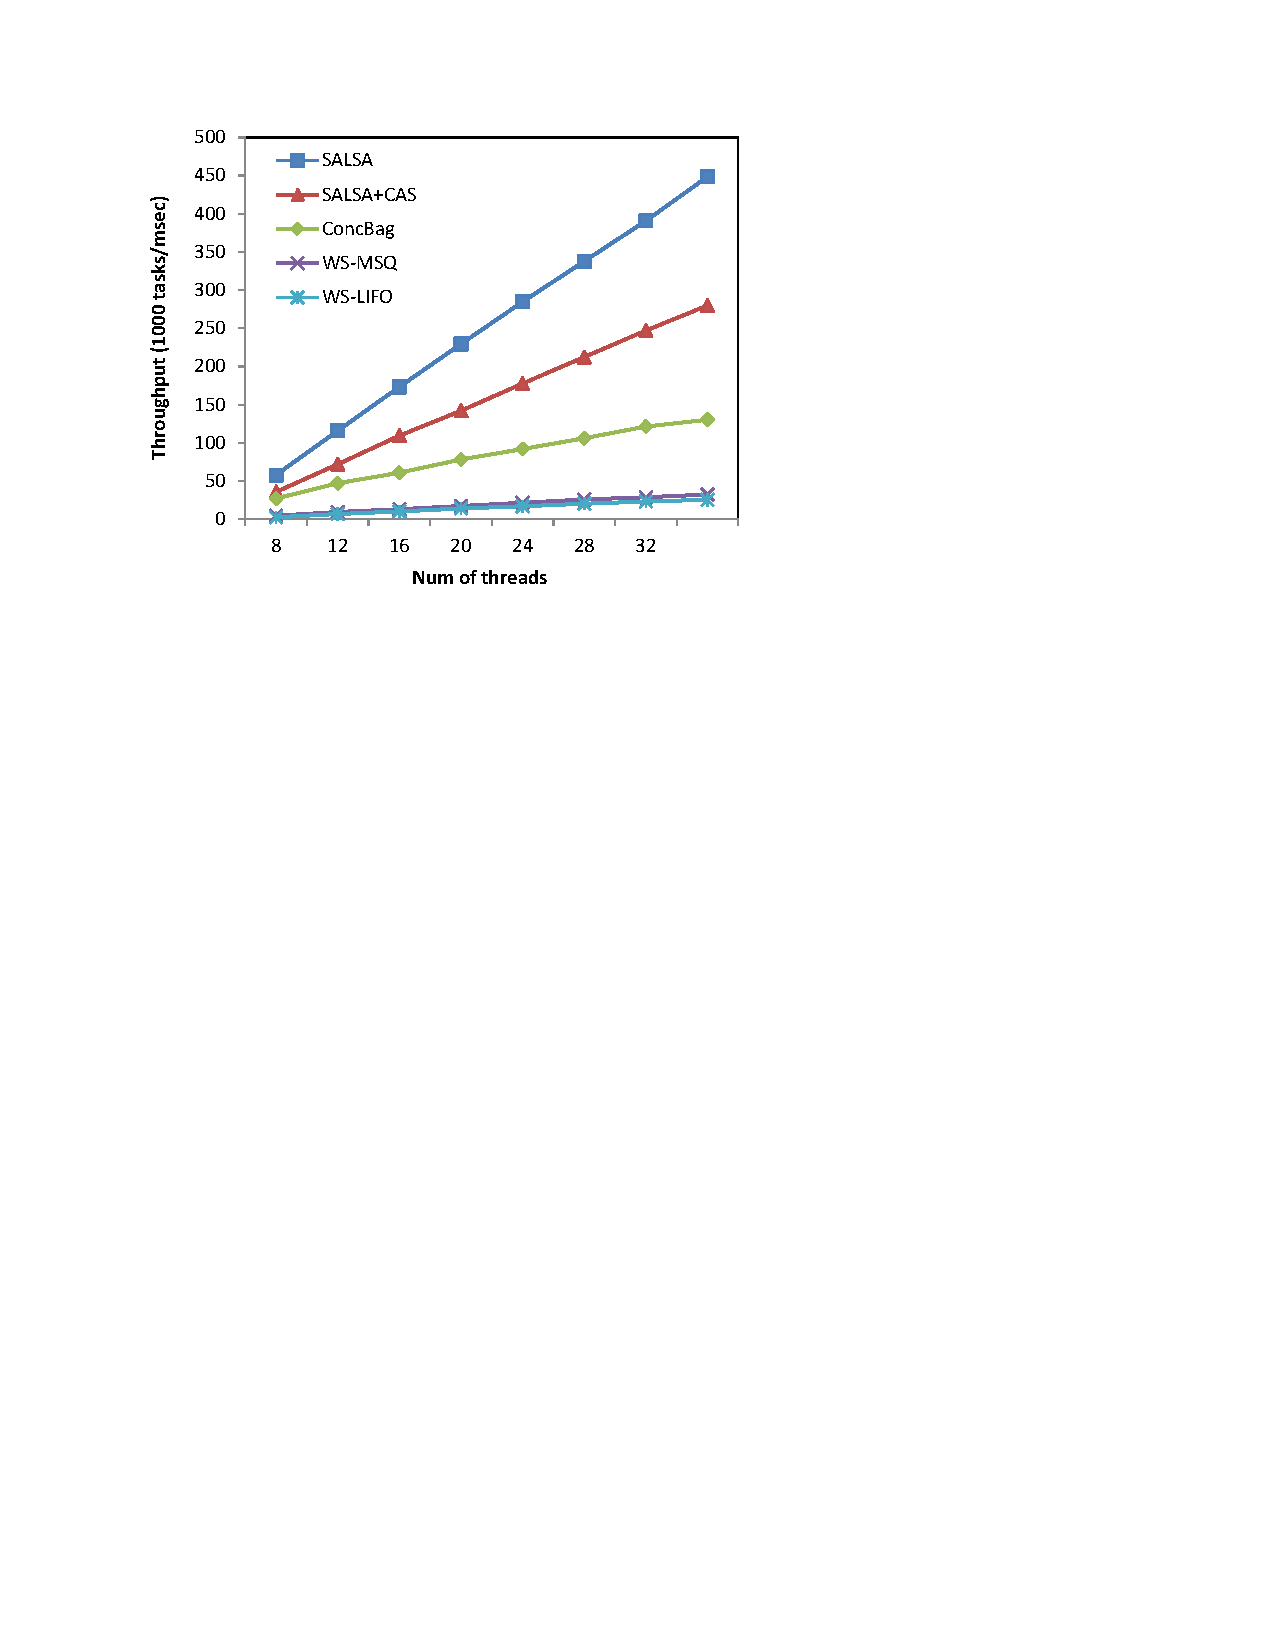
\includegraphics[width=0.45\textwidth]{figures/n-n-throughput}
    \label{fig:n-n-throughput}
  }
  \subfigure [\scriptsize{System throughput -- variable prod-cons ratio.}] {
    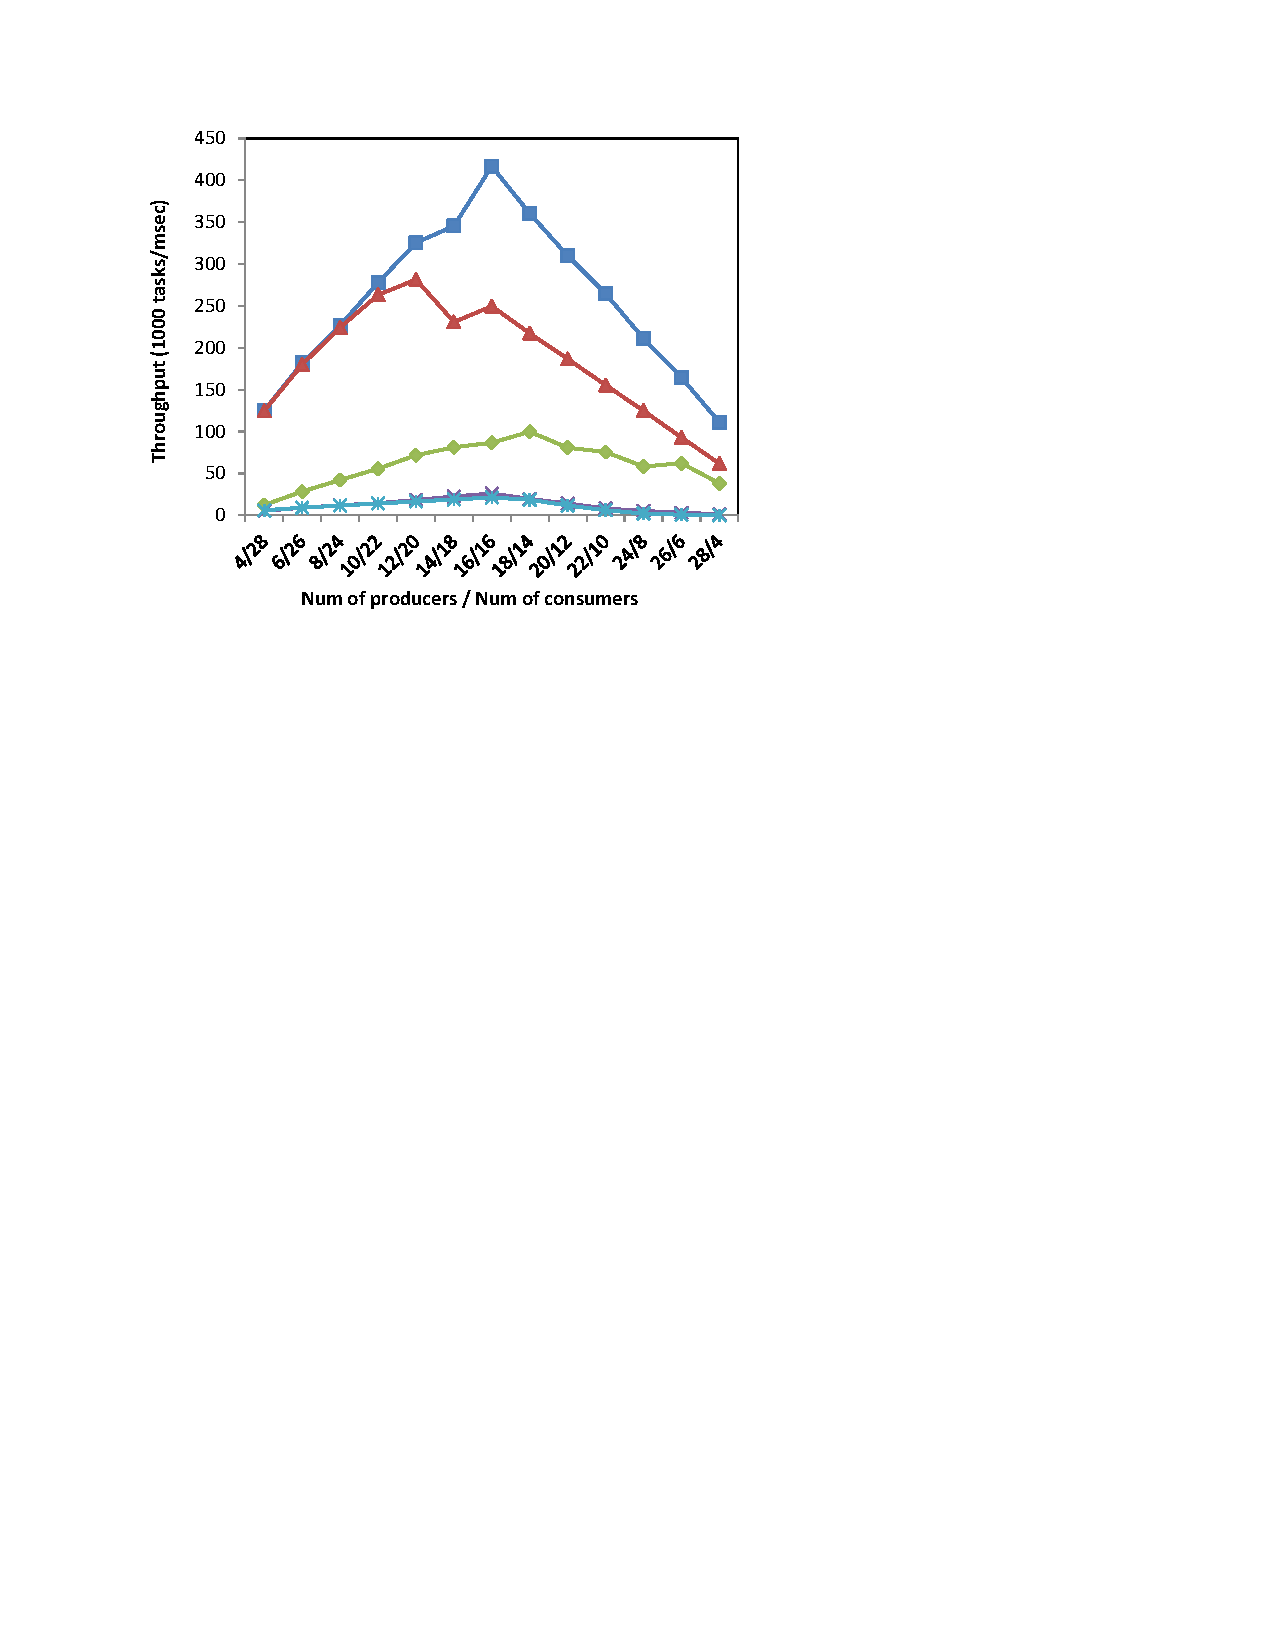
\includegraphics[width=0.45\textwidth]{figures/prod-cons-fig}
    \label{fig:prod-cons-fig}
  }
	\caption{\footnotesize{System throughput for various ratios of producers and consumers. WS-SALSA scales linearly with the number of threads -- in the $16/16$ workload, it is $\times20$ faster than WS-MSQ with WS-LIFO, and more than $\times5$ faster than the Concurrent Bags algorithm. In tests with equal number of producers and consumers the differences among work-stealing alternatives are mainly explained by the consumption algorithm efficiency (stealing rate is low and does not influence on the performance). In contrast, in Concurrent Bags algorithm every {\bf consume()} operation implies stealing, which causes the sub-linear scalability of ConcBags.
}}
	\label{fig:throughput}
\end{figure}

Figure~\ref{fig:throughput} demonstrates system throughput of the compared algorithms for the workloads with various numbers of producers and consumers. 
Figure~\ref{fig:n-n-throughput} shows throughput dynamics when the number of producers is equal to the number of consumers. WS-SALSA \emph{scales linearly} as the number of threads grows to $32$ (the number of physical cores in the system), and it clearly outperforms all other competitors. In the $16/16$ workload, WS-SALSA is $\times20$ faster than WS-MSQ with WS-LIFO, and more than $\times5$ faster than the Concurrent Bags algorithm. 

The performance of ConcBags in our experiments differs from the one presented by Sundell et al.~\cite{Sundell:2011:LAC:1989493.1989550}. 
While in the original paper ConcBags' throughput drops by the factor of $3$ when the number of threads increases from $4$ to $24$, in our tests the performance of ConcBags increases with the number of threads. The reasons for the scalability of our implementation and non-scalability of the original one can be related to different memory allocators, hardware architectures and engineering optimizations. %In any case, both implementations provide the performance of tens of thousands of task retrievals in msec for multiple producers and consumers. 

The stealing rate in the workloads with equal number of producers and consumers remains low; hence, consumers in our work-stealing framework work independently most of the time. The differences in the performance of the competitors are thus explained by the {\bf consume()} algorithm efficiency only. 
For example, WS-SALSA is $\times1.7$ faster than WS-SALSAwCAS because of the fast-path consumption technique that does not use strong atomic operations. 
In contrast, in Concurrent Bags algorithm, which is not based on per-consumer pools, every {\bf consume()} operation implies stealing that causes contention among consumers, which is the reason for sub-linear scalability of ConcBags.

Figure~\ref{fig:prod-cons-fig} shows system throughput of the algorithms for various ratios between producers and consumers. The optimal behavior of all algorithms is achieved when the number of producers is equal to the number of consumers; SALSA outperforms other alternatives for all possible producer-consumer ratios. 

\begin{figure}[htb]
	\centering
  \subfigure [\scriptsize{System throughput -- 1 Producer, N consumers.}] {
    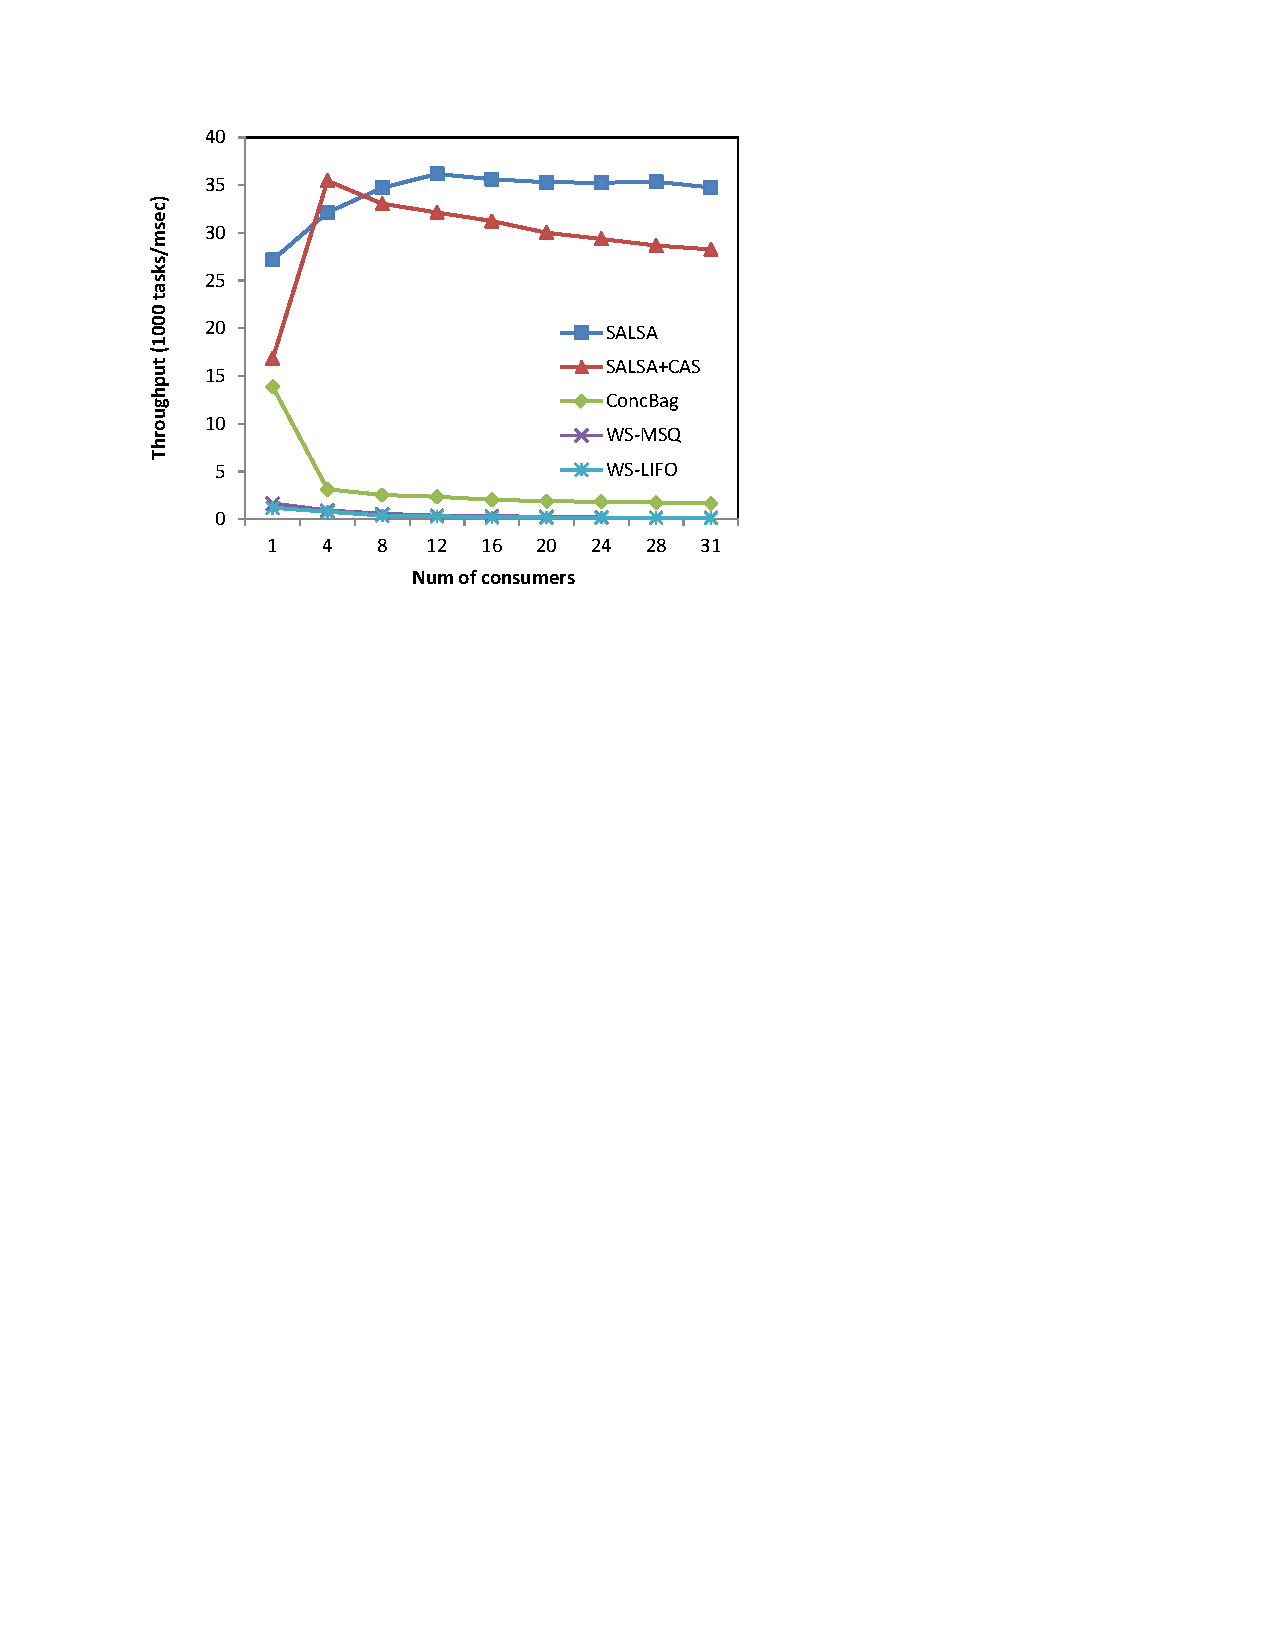
\includegraphics[width=0.45\textwidth]{figures/1-n-throughput}
    \label{fig:1-n-throughput}
  }
  \subfigure [\scriptsize{CAS operations per task retrieval -- 1 Producer, N consumers.}] {
    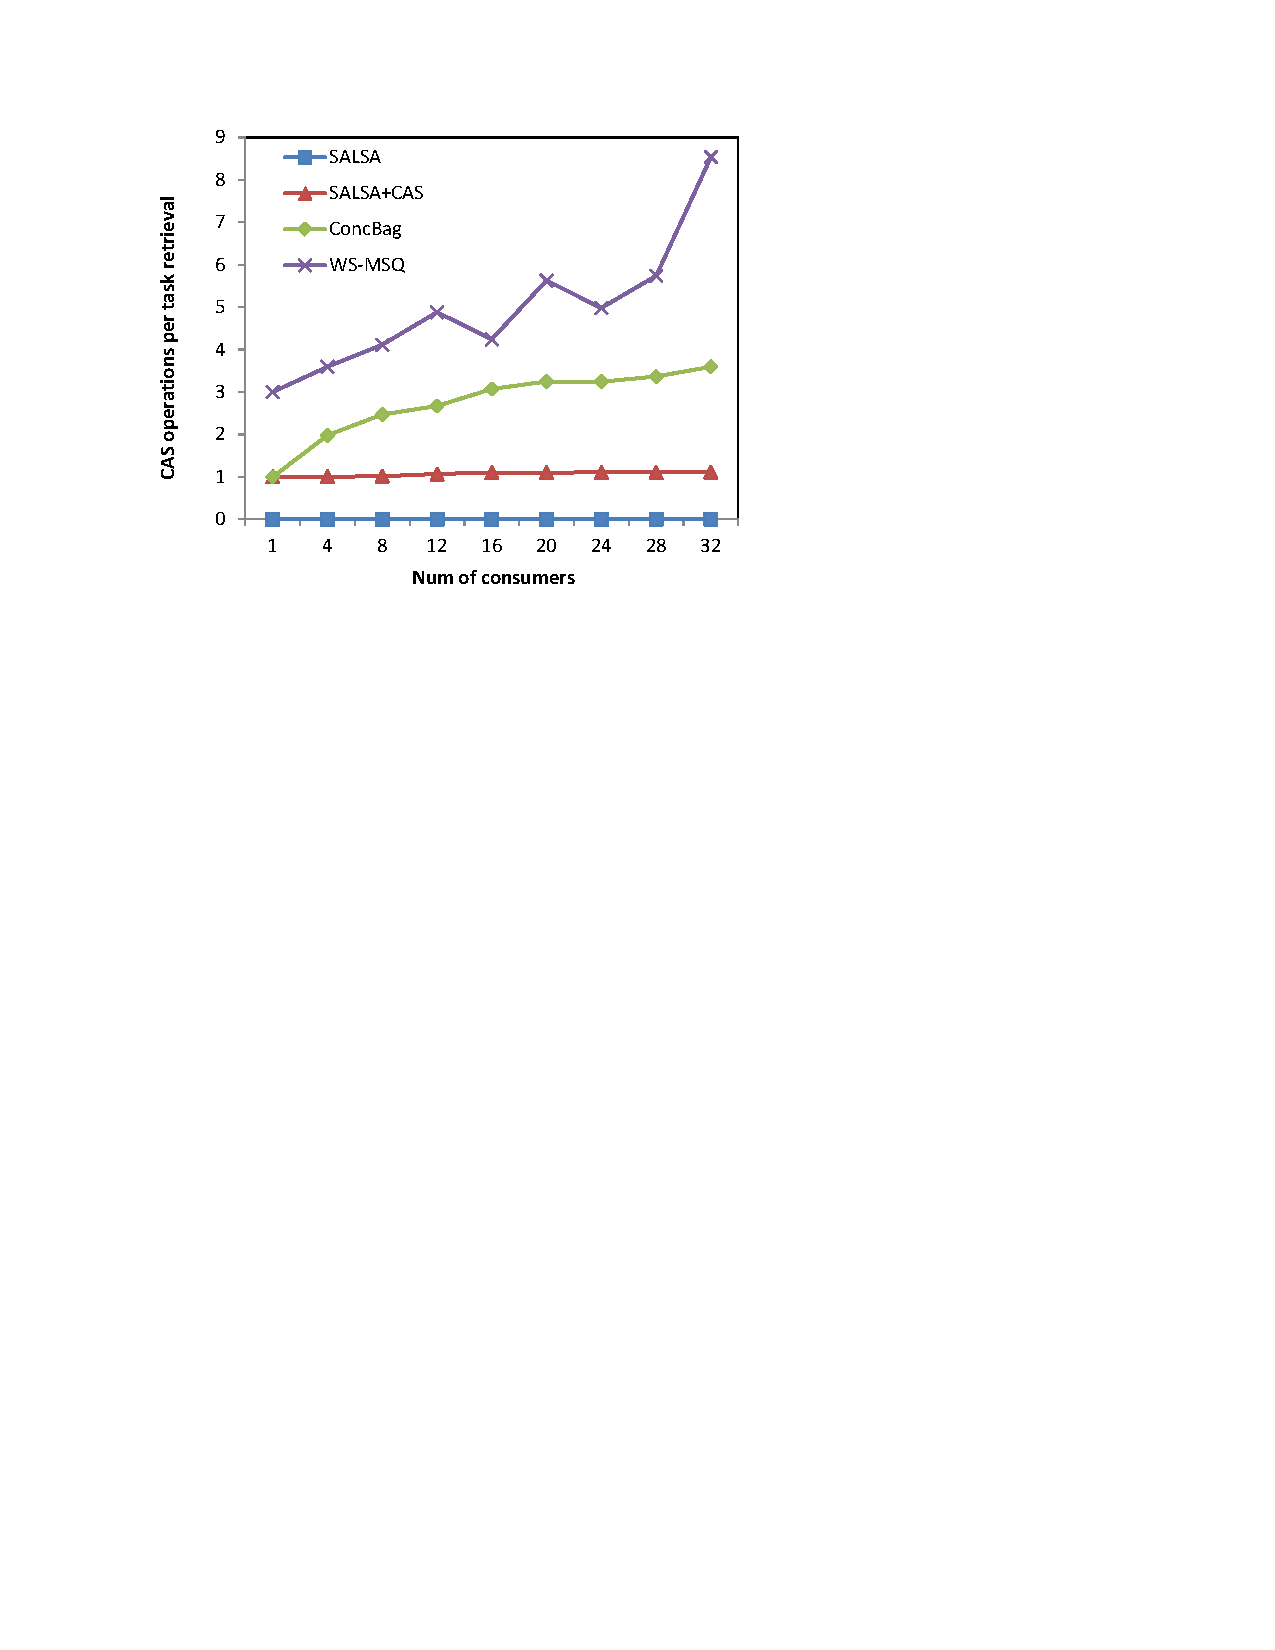
\includegraphics[width=0.45\textwidth]{figures/1-n-cas}
    \label{fig:1-n-cas}
  }
	\caption{\footnotesize{System behavior in the workloads with a single producer and multiple consumers. 
	Both WS-SALSA and WS-SALSAwCAS tolerate high stealing rates. The throughput of other algorithms drops by the factor of $10$ because of the increased contention among consumers trying to steal tasks from the same pool.}}
	\label{fig:1-n-perf}
\end{figure}

We now evaluate the behavior of the compared pools in the scenarios with excessive stealing. To this end, we measure their performance in the workloads with a single producer and multiple consumers (see Figure~\ref{fig:1-n-perf}). 
Figure~\ref{fig:1-n-throughput} shows that both WS-SALSA and WS-SALSAwCAS tolerate high stealing rates. In contrast, the throughput of other algorithms drops by the factor of $10$ when the number of consumers raises from $1$ to $32$. 
This degradation is caused by the increased contention among consumers that try to steal tasks from the same pool. 
Figure~\ref{fig:1-n-cas} evaluates this contention by measuring the average number of CAS operations executed for a single task transfer (by both producers and consumers). While the number of CAS operations of SALSA remains close to $0$, both WS-MSQ and ConcBag suffer from severe CAS failure rate when the number of competing consumers increases. 

\subsection{Evaluation of SALSA Techniques}
\label{sec:eval-techniques}
\begin{figure}[htb]
	\centering
  \subfigure [\scriptsize{System throughput -- 1 Producer, N consumers.}] {
    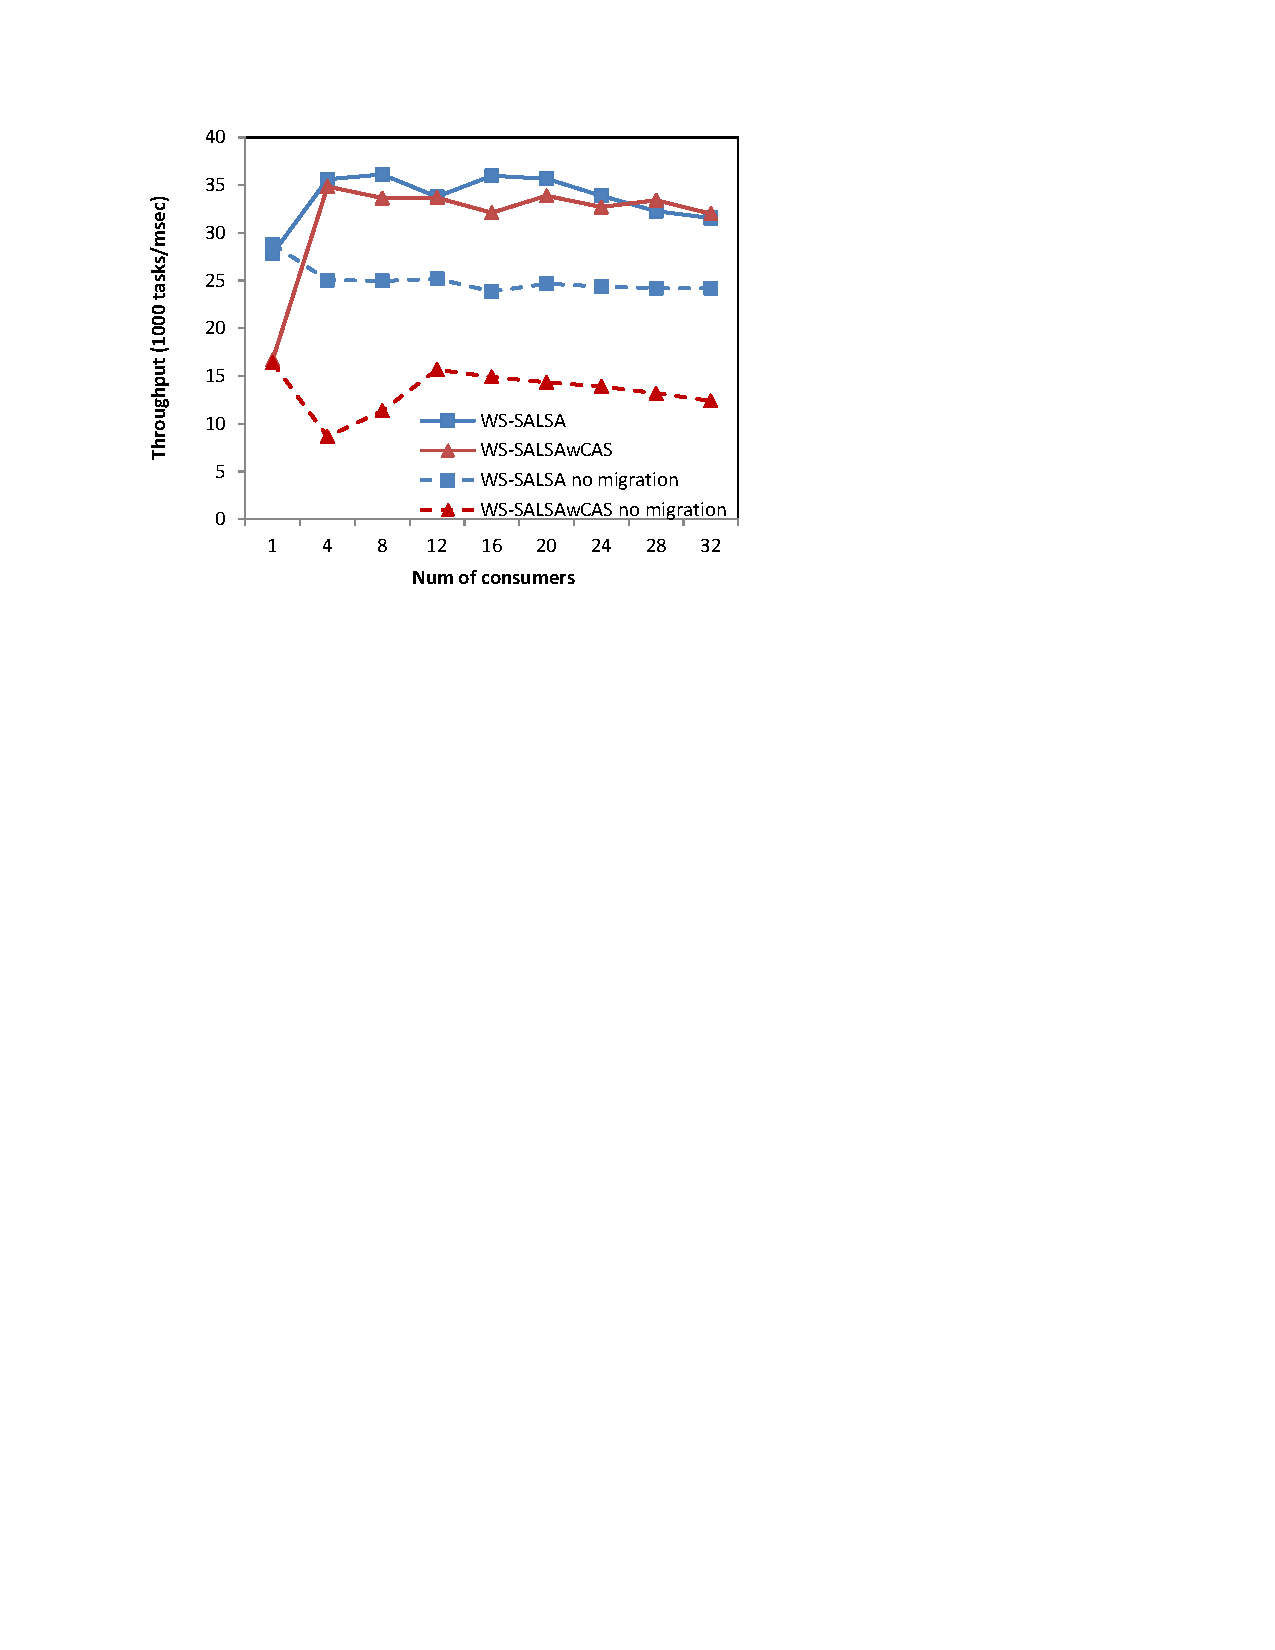
\includegraphics[width=0.45\textwidth]{figures/1-n-salsa}
    \label{fig:1-n-salsa-perf}
  }
  \subfigure [\scriptsize{CAS operations per task retrieval -- 1 Producer, N consumers.}] {
    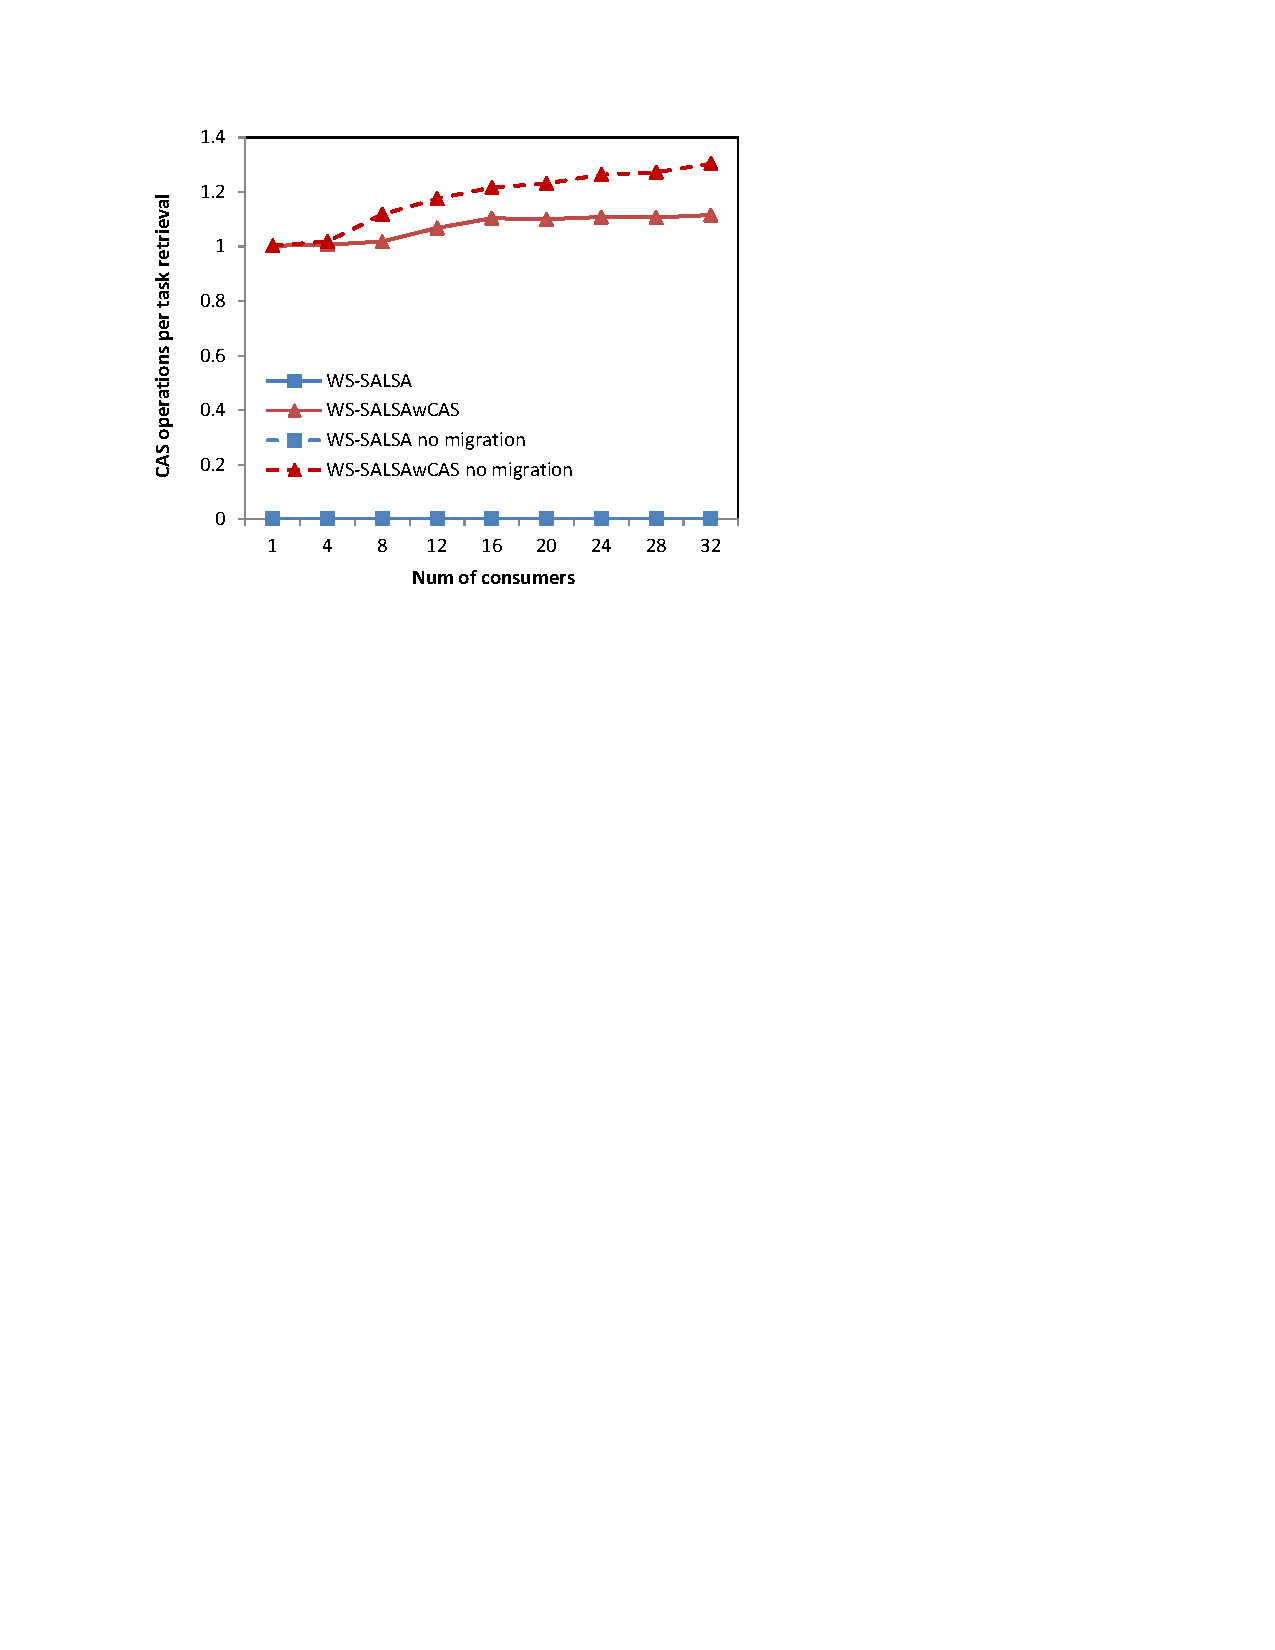
\includegraphics[width=0.45\textwidth]{figures/1-n-salsa-cas}
    \label{fig:1-n-salsa-cas}
  }
	\caption{\footnotesize{SALSA techniques in the workloads with a single producer and multiple consumers. The producers in our framework try to avoid inserting tasks to the overloaded consumers, thus decreasing stealing frequency (bold lines behave similarly). If this migration mechanism is disabled, stealing becomes prevalent and the chunk stealing technique becomes important (dashed lines behave differently). }}
	\label{fig:1-n-salsa}
\end{figure}
We now study empirically the influence of SALSA techniques for its performance. 
%
%\begin{wrapfigure}{r}{0.47\textwidth}
%  \vspace{-20pt}
%  \begin{center}
%    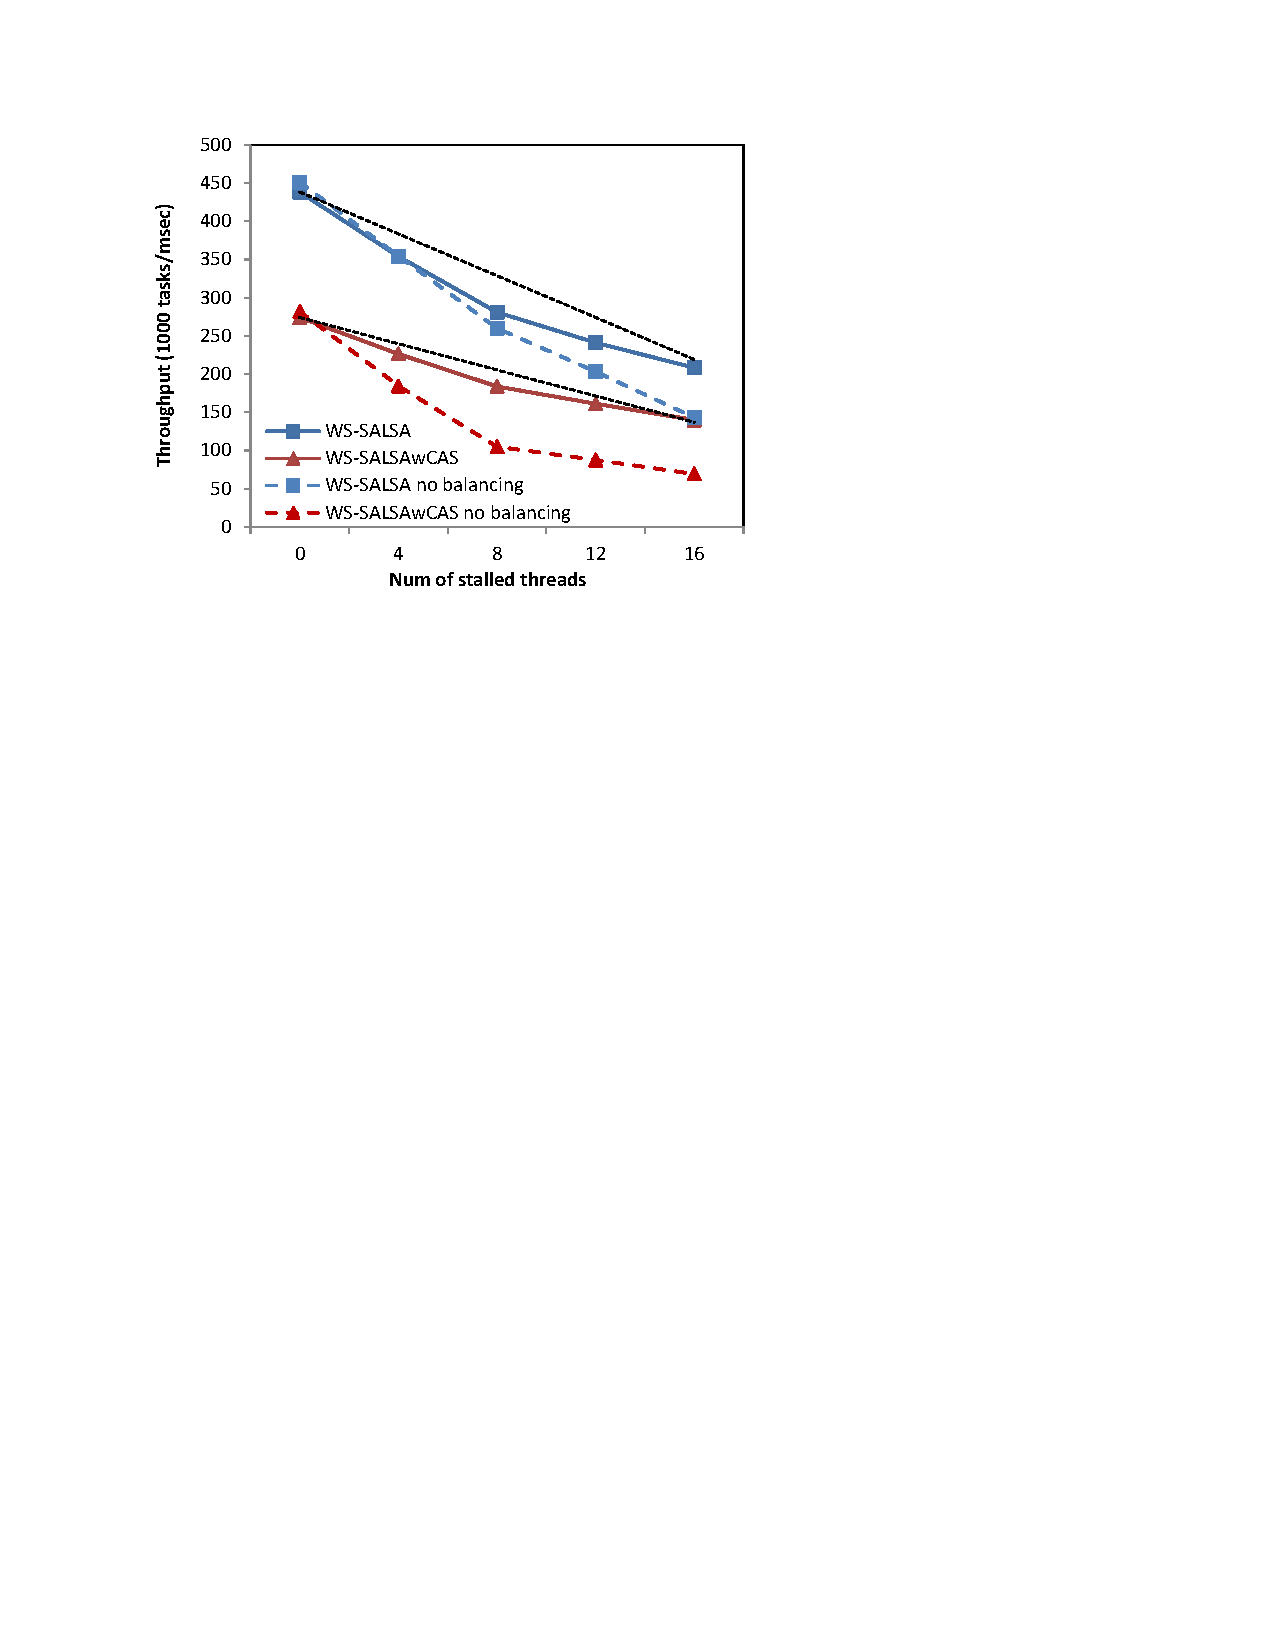
\includegraphics[width=0.45\textwidth]{figures/stalled-threads}
%  \end{center}
%  \vspace{-20pt}
%  \caption{\footnotesize{System throughput in a system with $16$ producers and $16$ consumers as a function of the number of stalled threads.}}
%  \vspace{-10pt}
%  \label{fig:stalled-threads}
%\end{wrapfigure}
%
%%
%%
%%\begin{figure}[htb]
%%	\centering
%%	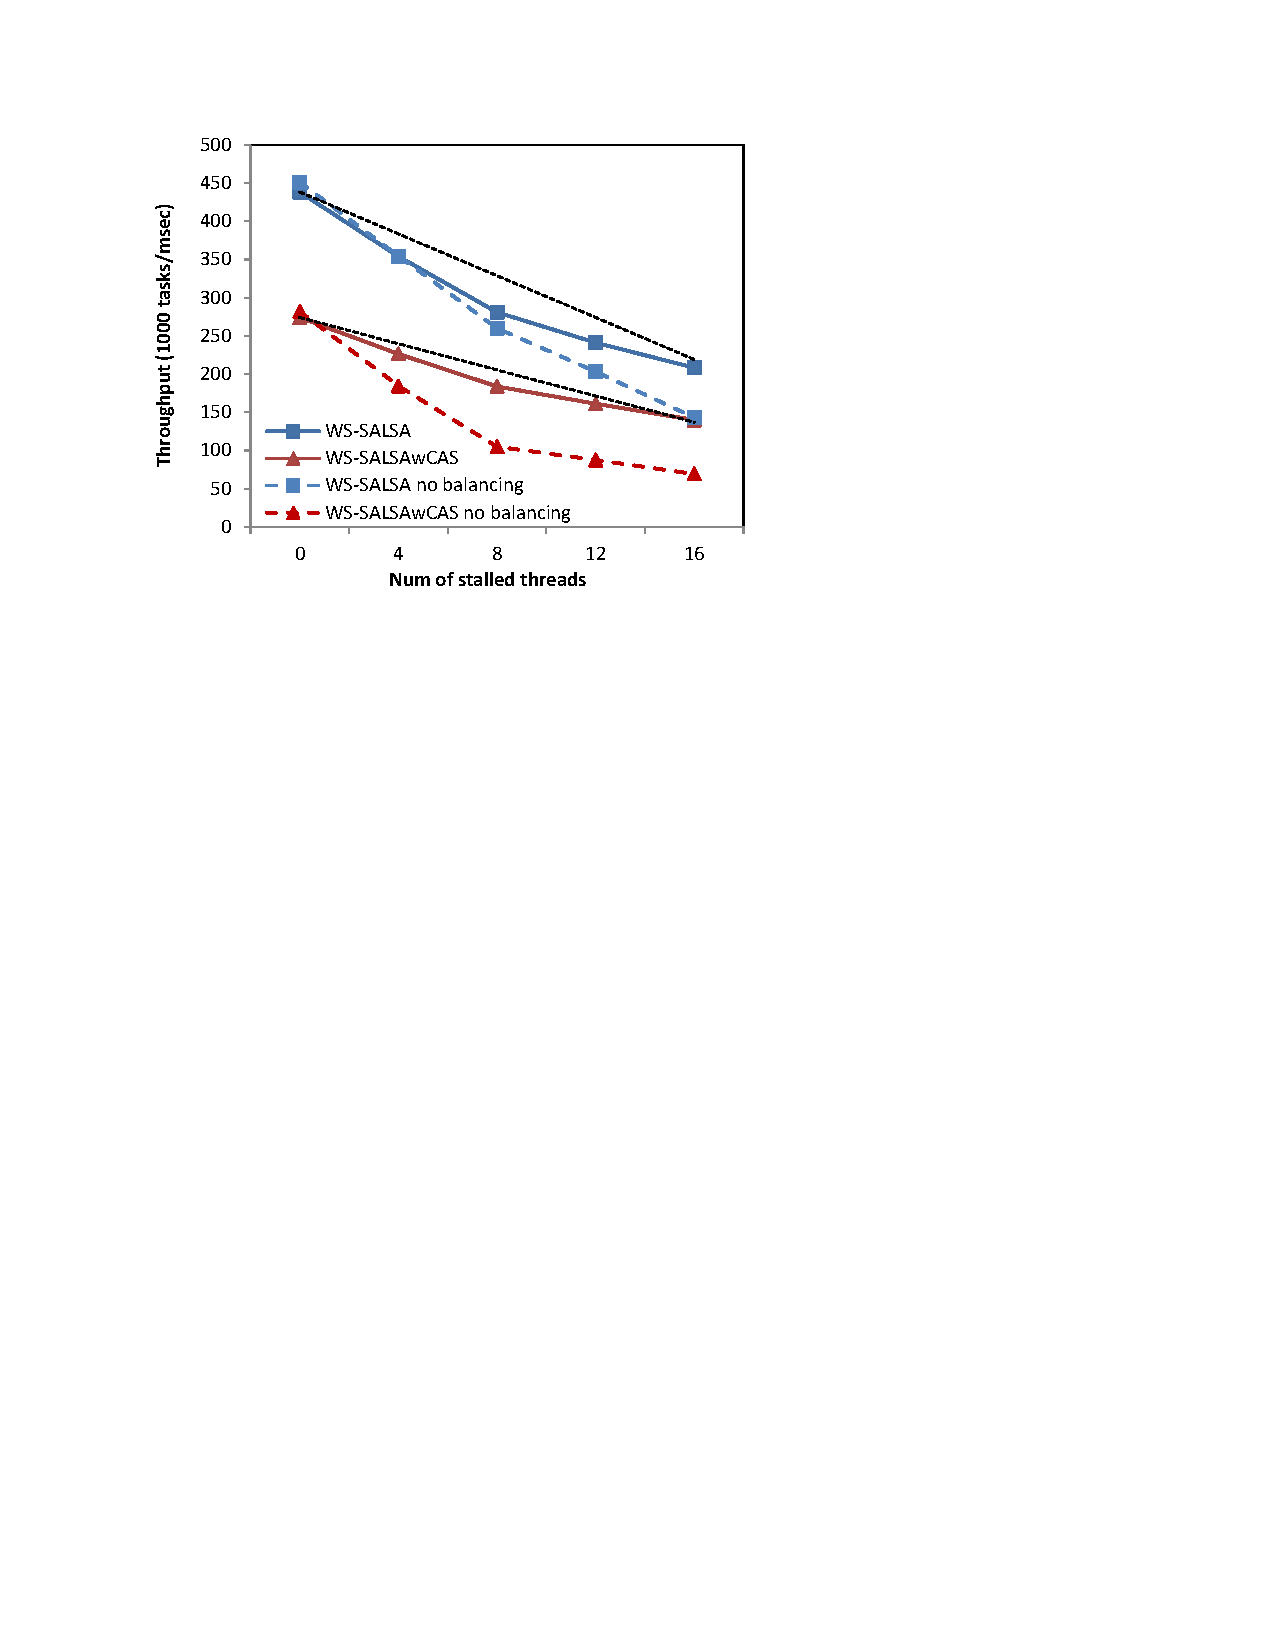
\includegraphics[width=0.45\textwidth]{figures/stalled-threads}
%%  \caption{\footnotesize{System throughput for different number of stalled threads (N/N workload). }}
%%	\label{fig:stalled-threads}
%%\end{figure}
%
%producer migration -- robustness against unpredictable stalls
%
%\begin{figure}[htb]
%	\centering
%	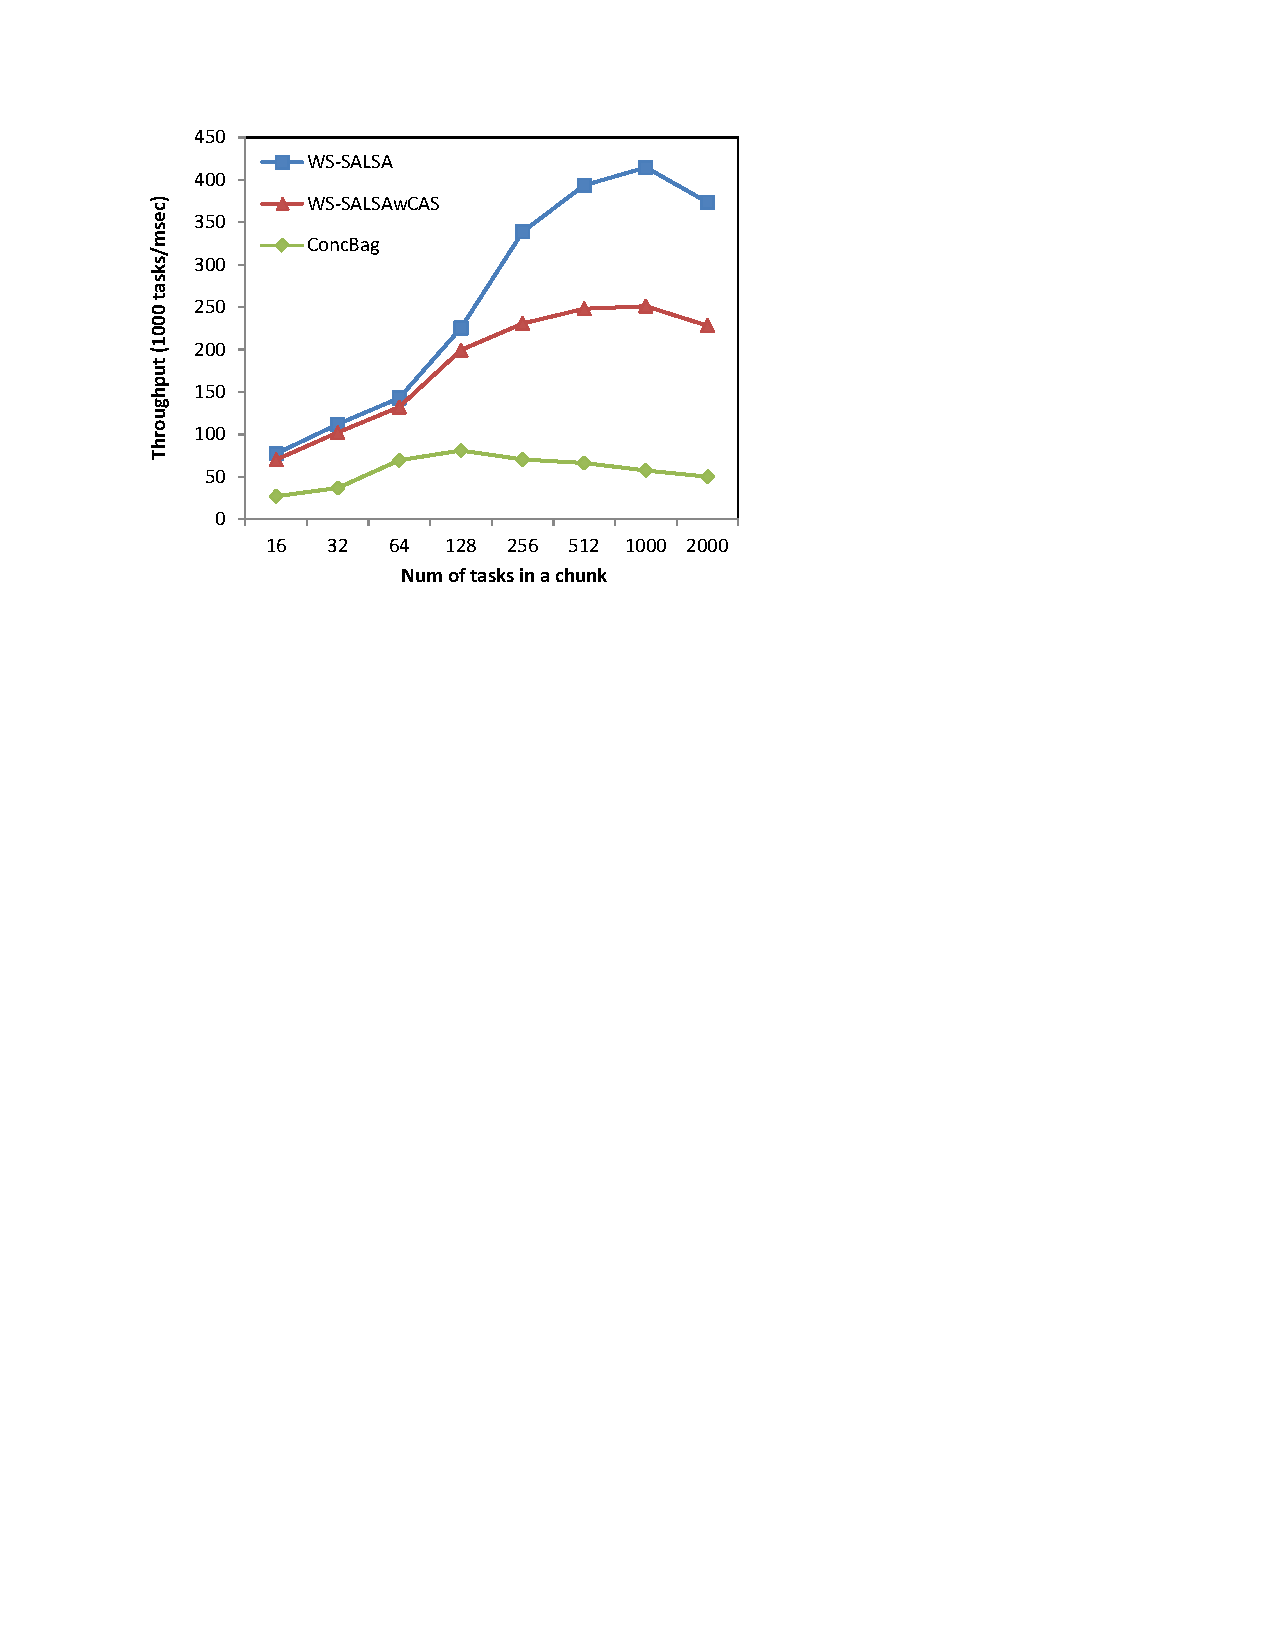
\includegraphics[width=0.45\textwidth]{figures/chunk-size}
%  \caption{\footnotesize{System throughput as a function of chunk size. }}
%	\label{fig:chunk-size}
%\end{figure}